\chapter{Experiments on Predicting Liver Fat}
\label{chap:cap-experiments}

This chapter records the experiments run to predict the controlled attenuation parameter (CAP; NHANES variable LUXCAPM, dB/m), the FibroScan measure of liver fat that the patient-state model of HepatoTwin estimates from routine data. Fifty-one experiments, run between 5 September and 22 October 2026, varied the learning algorithm, the inputs, the training weights, the treatment of the target, the training data and the evaluated population. Section~\ref{sec:exp-protocols} defines how results were measured; Section~\ref{sec:exp-list} lists every experiment and its result; Section~\ref{sec:exp-final} describes the model that was selected and its performance; Section~\ref{sec:exp-plateau} explains why $R^2$ stops rising; and Section~\ref{sec:exp-compare} compares the result with published models. Section~\ref{sec:exp-summary} summarises the chapter.

%--------------------------------------------------------------------
\section{Evaluation Protocols}
\label{sec:exp-protocols}

The cohort comprised NHANES participants with a complete elastography examination (LUAXSTAT\,=\,1) and an observed CAP, aged 12 to 80 years. $R^2$ is the share of the variation in measured CAP that the predictions explain on participants the model was not trained on. Three protocols were used as the work progressed (Table~\ref{tab:protocols}). Because each protocol scores a different set of participants, $R^2$ values from different protocols are not directly comparable, and every result below is labelled with its protocol.

\begin{table}[t]
\centering
\small
\caption{Evaluation protocols.}
\label{tab:protocols}
\begin{tabularx}{\textwidth}{@{}l Y Y@{}}
\toprule
Code & Design & Used for \\
\midrule
P1 & 9,021 participants (2017--March 2020) split once 80/20 (seed 42) into 7,216 development and 1,805 test participants; model choice by five-fold cross-validation on the development set (P1-CV), test results as P1-test. & September and early October. The test set was examined repeatedly, so P1-test is an internal comparison. \\
P2 & All 9,021 participants, five-fold cross-validation (seed 42); $R^2$ on the pooled out-of-fold predictions. Baseline 0.5135. & Model families and new data (October). \\
P3 & 15,300 participants from both FibroScan cycles (2017--2020 and 2021--2023). A 20\% test set (3,060, stratified by cycle, seed 42) set aside first; model choice by five-fold cross-validation on the remaining 12,240 (P3-CV); test set scored once (P3-test). & Combined model and final selection. \\
\bottomrule
\end{tabularx}
\end{table}

Outcomes are labelled \emph{Adopted} (carried into the model), \emph{Small gain} (below about 0.01, not or not fully adopted), \emph{No gain}, \emph{Worse} and \emph{Diagnostic} (an analysis explaining the model's behaviour rather than a candidate model).

%--------------------------------------------------------------------
\section{Experiments}
\label{sec:exp-list}

The experiments fall into six phases. Each phase was prompted by the findings of the one before it: once changes to the model stopped helping, the work turned to the target variable, then to new data, and finally to the population in which the model is used.

\subsection{Phases 1 and 2: baselines, tuning and inputs}

The first models used 14 inputs: age, sex, race and ethnicity, BMI, waist circumference, ALT, AST, HbA1c, total and HDL cholesterol, and day-one dietary energy, protein, carbohydrate and fat (Table~\ref{tab:phase12}).

\begin{table}[t]
\centering
\small
\caption{Phase 1 and 2 experiments: baselines, tuning and inputs.}
\label{tab:phase12}
\begin{tabularx}{\textwidth}{@{}l Y Y l@{}}
\toprule
ID & Experiment & Result & Outcome \\
\midrule
E1 & Baseline XGBoost, 14 inputs & P1-test $R^2$ 0.491; RMSE 44.5\,dB/m & Adopted \\
E2 & XGBoost against linear regression and random forest & P1-test 0.491; 0.488; 0.486 & Small gain \\
E3 & Leakage-free preprocessing and a 40-setting search & Corrected baseline 0.485 $\rightarrow$ 0.506 (P1-test) & Adopted \\
E4 & 14, 19 and 28 inputs (extra blood tests) and 24 model variants & P1-CV 0.489 / 0.496 / 0.501; blend 0.502 & Small gain \\
E5 & Reproduction of a supplied model reporting 0.535 & On its own split: supplied 0.535, ours 0.541; on our split: 0.511 and 0.514 & Diagnostic \\
E6 & 36 raw inputs plus 10 engineered features & P1-CV 0.506; P1-test 0.515 & Small gain \\
\bottomrule
\end{tabularx}
\end{table}

A linear model came close to the tree ensemble (E2), a first sign that the signal is mostly additive and driven by body size. The first clear gain came from fitting imputation inside each fold and tuning the trees (E3). Shallow trees, a low learning rate and row subsampling reduce overfitting when the target is noisy. Rather than coming from a better model, experiment E5 showed that a supplied model's higher $R^2$ came from an easier test split, and that a single 20\% split moves $R^2$ by about $\pm 0.03$.

\subsection{Phase 3: features, weighting and learners}

Phase 3 tested whether reshaping the inputs or the training weights could help (Table~\ref{tab:phase3}). None changed $R^2$ by more than 0.003.

\begin{table}[t]
\centering
\small
\caption{Phase 3 experiments: feature ablations and weighting (P1-CV).}
\label{tab:phase3}
\begin{tabularx}{\textwidth}{@{}l Y Y l@{}}
\toprule
ID & Experiment & Result & Outcome \\
\midrule
E7 & Engineered-feature ablation & 0.5035 / 0.5048 / 0.5032 / 0.5036 & Small gain \\
E8 & Single ratios (WHtR, AST/ALT, TG/HDL, TC/HDL) & 0.5022--0.5038 against 0.5035 & No gain \\
E9 & LDL cholesterol & 0.5036 $\rightarrow$ 0.5020 / 0.5030 & No gain \\
E10 & Recursive feature elimination, 46 to 10 inputs & 46: 0.504; 25: 0.508; 15: 0.501; 10: 0.485 & No gain \\
E11 & Histogram gradient boosting & 0.486 against XGBoost 0.505 & Worse \\
E12 & Up-weighting extreme CAP values & 0.505 $\rightarrow$ 0.500 / 0.494 / 0.488 & Worse \\
\bottomrule
\end{tabularx}
\end{table}

About 20 to 25 inputs carry nearly all the signal, led by waist circumference, waist-to-height ratio and BMI (E10). Derived scores such as the Fatty Liver Index re-express inputs that the trees can already combine (E7--E8).

\subsection{Phase 4: the target and other model families}

Phase 4 first examined the target itself (Table~\ref{tab:phase4a}) and then tried other model families and target treatments (Table~\ref{tab:phase4b}).

\begin{table}[t]
\centering
\small
\caption{Phase 4 diagnostics of the target.}
\label{tab:phase4a}
\begin{tabularx}{\textwidth}{@{}l Y Y l@{}}
\toprule
ID & Experiment & Result & Outcome \\
\midrule
E13 & Residuals by CAP range (P2) & Slope of prediction on actual 0.51; bias +44\,dB/m below 200 and $-$67\,dB/m above 390 & Diagnostic \\
E14 & CAP ceiling audit & 129 of 9,021 (1.4\%) exactly 400\,dB/m & Diagnostic \\
E15 & Refit without CAP\,=\,400 & $R^2$ 0.506 $\rightarrow$ 0.488; RMSE 44.3 $\rightarrow$ 43.7\,dB/m & No gain \\
E16 & Performance by probe & Within-probe $R^2$: M 0.419, XL 0.278 & Diagnostic \\
\bottomrule
\end{tabularx}
\end{table}

Predictions are pulled towards the mean of about 255\,dB/m (E13): the inputs cannot separate very lean or very fatty livers from average ones. The device truncates CAP at 400\,dB/m (E14), but too few readings are affected to limit $R^2$, and removing them lowers $R^2$ because the outcome variance shrinks (E15).

\begin{table}[t]
\centering
\small
\caption{Phase 4 experiments: model families and target treatments.}
\label{tab:phase4b}
\begin{tabularx}{\textwidth}{@{}l Y Y l@{}}
\toprule
ID & Experiment & Result & Outcome \\
\midrule
E17 & Probe type (M or XL) as an input & 0.5062 $\rightarrow$ 0.5112 & Small gain$^{a}$ \\
E18 & XL examinations weighted 1.5$\times$ and 2$\times$ & 0.5112 $\rightarrow$ 0.5080 / 0.5018 & Worse \\
E19 & CatBoost (P2) & 0.5093 against XGBoost 0.5135 & No gain \\
E20 & Steatosis-class probabilities fed to the regressor & 0.5116 / 0.5129 & No gain \\
E21 & Linear recalibration of predictions & 0.5127 & No gain \\
E22 & Quantile (median) regression & 0.503 against 0.506; 80\% interval covers 74.7\% & No gain \\
E23 & Fold-local Lasso and RFE selection & 0.499; 0.504 & No gain \\
E24 & Extra Trees, random forest, ridge & 0.500; 0.498; 0.482 & No gain \\
E25 & Neural network (128, 64) & 0.453 & Worse \\
E26 & Stacking with a ridge meta-learner & 0.506 $\rightarrow$ 0.509 & Small gain \\
E27 & Steatosis classification & Binary AUC 0.862; four-class macro F1 0.439 & Adopted \\
E28 & HbA1c ablation & Not completed & -- \\
\bottomrule
\end{tabularx}
\par\smallskip
{\footnotesize $^{a}$Not used: probe type is recorded during the FibroScan examination itself.}
\end{table}

Every model family reached the same ceiling (E19, E24--E26). The binary classification of steatosis (E27) performed well and became the second output of the model; the four-class task failed for the middle grades, which span only 20 and 12\,dB/m, less than the model error.

\subsection{Phase 5: additional data}

Phase 4 indicated that the limit lay in the information available, not in the model, so Phase 5 added NHANES data not used before (Table~\ref{tab:phase5}). Elastography fields and self-reported liver conditions were never used as inputs, because they would leak the target.

\begin{table}[t]
\centering
\small
\caption{Phase 5 experiments: additional data.}
\label{tab:phase5}
\begin{tabularx}{\textwidth}{@{}l Y Y l@{}}
\toprule
ID & Experiment & Result & Outcome \\
\midrule
E29 & About 80 more NHANES variables (insulin, CRP, blood count, blood pressure, questionnaires, prescriptions) & 0.5135 $\rightarrow$ 0.5239 (128 inputs, P2) & Small gain \\
E30 & Learning curve (25--100\% of training data) & 0.488; 0.501; 0.511; 0.512 & Diagnostic \\
E31 & 2021--2023 FibroScan cycle (6,279 participants) & 0.5135 $\rightarrow$ 0.5170 & Small gain \\
E32 & DXA visceral and subcutaneous fat (3,307) & 0.5094 $\rightarrow$ 0.5168 & Small gain \\
E33 & Measurement noise within an examination & About 3.7\% of CAP variance & Diagnostic \\
E34 & Upper bound with FibroScan-derived inputs & 0.518 $\rightarrow$ 0.524 (probe), 0.529 (stiffness) & Diagnostic \\
E35 & Combined model: both cycles, 81 inputs, reliability weights (P3) & P3-test 0.480 $\rightarrow$ 0.493; P3-CV 0.520 & Adopted \\
E36 & Cohort filters & All 0.518; IQR $<$ 40 and ages 12--59: 0.584 & Diagnostic \\
E37 & Performance by age group & 12--17: 0.43; 18--39: 0.54; 40--59: 0.49; 60+: 0.41 & Diagnostic \\
E38 & Improving the 60+ group & 0.405 $\rightarrow$ 0.394--0.408 & No gain \\
E39 & Calibrated classifiers, CAP $\geq$ 248 and $\geq$ 280 & AUC 0.856 and 0.868; calibration error 0.025 $\rightarrow$ 0.018 & Adopted \\
\bottomrule
\end{tabularx}
\end{table}

The largest single gain in the record, $+0.010$, came from the extra NHANES variables (E29), mainly insulin resistance and diabetes and weight history. The learning curve was flat (E30), so a second cycle of 6,279 participants added only 0.004 (E31). Even visceral fat measured directly by DXA, the strongest known correlate of liver fat, added only 0.007 (E32), and inputs taken from the FibroScan examination itself reached only 0.53 (E34). The combined model of E35 pooled both cycles and down-weighted less reliable examinations; it was adopted.

\subsection{Phase 6: target population and lean participants}

The cohort filters of E36 showed that $R^2$ is highest among participants aged 12 to 59 with a reliable examination (CAP interquartile range below 40\,dB/m). In this group the error itself falls (RMSE 43.6 $\rightarrow$ 41.6\,dB/m) while the spread of CAP does not shrink, so the higher $R^2$ reflects better predictions, not an easier outcome. On the supervisor's advice this group was adopted as the model's scope, and Phase 6 tried to reach 0.60 within it (Table~\ref{tab:phase6}).

\begin{table}[t]
\centering
\small
\caption{Phase 6 experiments within the scope (P3-CV; reference 0.5945).}
\label{tab:phase6}
\begin{tabularx}{\textwidth}{@{}l Y Y l@{}}
\toprule
ID & Experiment & Result & Outcome \\
\midrule
E40 & Training only on the scope; scope weighted 3$\times$; ages 12--59 only & 0.5845; 0.5921; 0.5883 & Worse \\
E41 & Habitual diet from the 24-hour recall & 0.5930 & No gain \\
E42 & Medical history and prescription count & 0.5949 & No gain \\
E43 & Fasting subsample only & 0.597 against 0.592 (test: 0.550 against 0.560) & No gain \\
E44 & Median imputation with indicators; MICE & 0.5961; 0.5938 & No gain \\
E45 & Pseudo-Huber loss; absolute-error loss & 0.5940; 0.5893 & No gain \\
E46 & Five further tree settings & 0.5915--0.5960 & Adopted$^{b}$ \\
E47 & Ensembles of 2--5 variants & Best 0.5969 & Small gain \\
E48 & Lean-only classifier (BMI $<$ 28) & Lean AUC 0.804 against 0.809 & Worse \\
E49--E51 & Lean weighting, non-obese training, blend & Lean AUC 0.807--0.808 & No gain \\
\bottomrule
\end{tabularx}
\par\smallskip
{\footnotesize $^{b}$The deepest setting had the highest test $R^2$ of all candidates (Section~\ref{sec:exp-final}).}
\end{table}

All variants scored between 0.584 and 0.597, a spread smaller than the variation between cross-validation folds (0.546 to 0.617). Training on the scope alone was worse than training on everyone (E40): participants outside the scope still carry information about how the inputs relate to CAP. Discrimination in lean participants (E48--E51) fell in every BMI band, and the Fatty Liver Index fell by a similar amount, because within a narrow BMI band the strongest predictor, body size, hardly varies.

%--------------------------------------------------------------------
\section{Final Model and Results}
\label{sec:exp-final}

The selected model is an XGBoost regressor \cite{chen2016xgboost} with 3,000 trees, depth 5, learning rate 0.005, minimum child weight 15 and column subsampling 0.4, trained on the 12,240 training participants of both FibroScan cycles. It uses 81 routine inputs (body measurements, standard blood tests, blood pressure and a short questionnaire) and six derived scores: waist-to-hip ratio, HOMA-IR, the triglyceride-glucose index, mean systolic and diastolic blood pressure, and one-year weight change. Examinations with a CAP interquartile range of 40\,dB/m or more are down-weighted (weight 40/IQR, at least 0.25) rather than dropped. Two isotonic-calibrated classifiers estimate the probability that CAP is at least 248 and at least 280\,dB/m.

The tree settings were chosen by scoring each of the 15 Phase 6 candidates on the in-scope members of the held-out test set; the deepest setting scored highest (0.5622 against 0.5582 for the reference). It also has the highest full-population cross-validation $R^2$ of the 12 settings compared, and repeated cross-validation, which played no part in the choice, confirms the gain (0.593 against 0.590). Because the test set informed the choice, the test figures are slightly optimistic.

\begin{table}[t]
\centering
\small
\caption{Selected model on the held-out test set (P3-test). The reference uses the 36 core inputs on the same participants.}
\label{tab:final-test}
\begin{tabular}{@{}l r r r r@{}}
\toprule
Test group & $n$ & $R^2$ & Reference $R^2$ & RMSE (dB/m) \\
\midrule
Scope: ages 12--59, reliable reference & 1,236 & 0.562 & 0.553 & 41.4 \\
\quad Ages 12--17 & 209 & 0.498 & 0.482 & 36.2 \\
\quad Ages 18--39 & 512 & 0.518 & 0.514 & 42.7 \\
\quad Ages 40--59 & 515 & 0.522 & 0.506 & 42.1 \\
Outside the scope: ages 12--59, all examinations & 2,040 & 0.515 & 0.511 & -- \\
Outside the scope: all participants & 3,060 & 0.496 & 0.487 & 43.5 \\
\bottomrule
\end{tabular}
\end{table}

Within the scope the held-out test $R^2$ is 0.562 (95\% bootstrap interval 0.517--0.601; Table~\ref{tab:final-test}), and 0.593 in five-fold cross-validation over all 15,300 participants repeated with three seeds. The value is lower within each age band than in the whole scope because CAP varies less within a band. Further checks did not change the picture (Table~\ref{tab:final-ci}): the result holds when weighted to the US population, and a model trained on 2017--2020 alone predicted the 2,415 in-scope participants of 2021--2023 with $R^2$ 0.578.

\begin{table}[t]
\centering
\small
\caption{Selected model within the scope, with 95\% bootstrap intervals.}
\label{tab:final-ci}
\begin{tabularx}{\textwidth}{@{}l Y Y Y@{}}
\toprule
Measure & Held-out test & Survey-weighted & Temporal (2021--2023) \\
\midrule
CAP $R^2$ & 0.562 (0.517--0.601) & 0.554 (0.493--0.609) & 0.578 (0.549--0.603) \\
CAP RMSE (dB/m) & 41.4 (39.3--43.6) & 42.6 (39.5--45.7) & 42.9 (41.4--44.5) \\
AUC, CAP $\geq$ 248 & 0.881 (0.863--0.899) & 0.877 (0.851--0.901) & 0.884 (0.870--0.896) \\
AUC, CAP $\geq$ 280 & 0.879 (0.860--0.898) & 0.878 (0.849--0.905) & 0.890 (0.878--0.904) \\
\bottomrule
\end{tabularx}
\end{table}

On the 1,100 in-scope test participants with every input to both scores, the CAP $\geq$ 248 classifier reached AUC 0.881 against 0.861 for the Fatty Liver Index \cite{bedogni2006fli} and 0.836 for the Hepatic Steatosis Index \cite{lee2010hsi}; the paired differences ($+0.020$ and $+0.046$) both exclude zero.

%--------------------------------------------------------------------
\section{Why $R^2$ Plateaus}
\label{sec:exp-plateau}

Nine independent lines of evidence show that the remaining variation in CAP cannot be explained by routine clinical measurements:

\begin{enumerate}
  \item Every algorithm tested (linear regression, random forest, Extra Trees, histogram boosting, XGBoost, CatBoost, a neural network and stacking) reaches $R^2$ between 0.45 and 0.52 on the same inputs (E2, E11, E19, E24--E26).
  \item Feature engineering, selection and ablation change $R^2$ by at most 0.003 (E7--E10, E23).
  \item The learning curve is flat: 6,279 additional participants add 0.004 (E30, E31; Figure~\ref{fig:learning-curve}).
  \item Direct DXA measurement of visceral fat adds 0.007 (E32).
  \item About 80 additional NHANES variables add 0.010 (E29).
  \item Even inputs taken from the FibroScan examination itself reach only 0.53 (E34).
  \item Noise within one examination is about 4\% of the CAP variance (E33), so the unexplained variance reflects real differences between people with similar measured profiles.
  \item Within the scope, every change to inputs, imputation, loss, tuning, training population and ensembling scored between 0.584 and 0.597, a spread smaller than the variation between folds (E40--E47).
  \item CAP is itself an imperfect measure of liver fat: two operators agree with a concordance of 0.82 \cite{ferraioli2021cap}, and CAP correlates with MRI-PDFF at $r = 0.66$ \cite{ahn2018cap}, sharing about 44\% of its variance with the reference measure.
\end{enumerate}

\begin{figure}[t]
\centering
\begin{minipage}{0.49\textwidth}
\centering
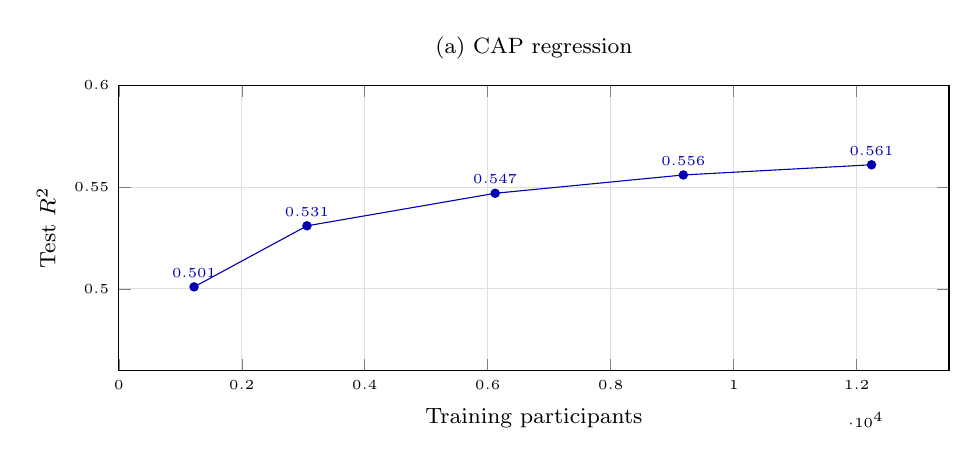
\begin{tikzpicture}
\begin{axis}[
  width=\linewidth, height=5.2cm,
  title={\footnotesize (a) CAP regression},
  xlabel={\footnotesize Training participants}, ylabel={\footnotesize Test $R^2$},
  xmin=0, xmax=13500, ymin=0.46, ymax=0.60,
  tick label style={font=\tiny}, label style={font=\footnotesize},
  grid=major, grid style={gray!25},
  nodes near coords={\pgfmathprintnumber[fixed,zerofill,precision=3]{\pgfplotspointmeta}},
  every node near coord/.append style={font=\tiny, above},
  ]
\addplot[blue!70!black, mark=*, mark size=1.5pt]
  coordinates {(1224,0.501) (3060,0.531) (6120,0.547) (9180,0.556) (12240,0.561)};
\end{axis}
\end{tikzpicture}
\end{minipage}\hfill
\begin{minipage}{0.49\textwidth}
\centering
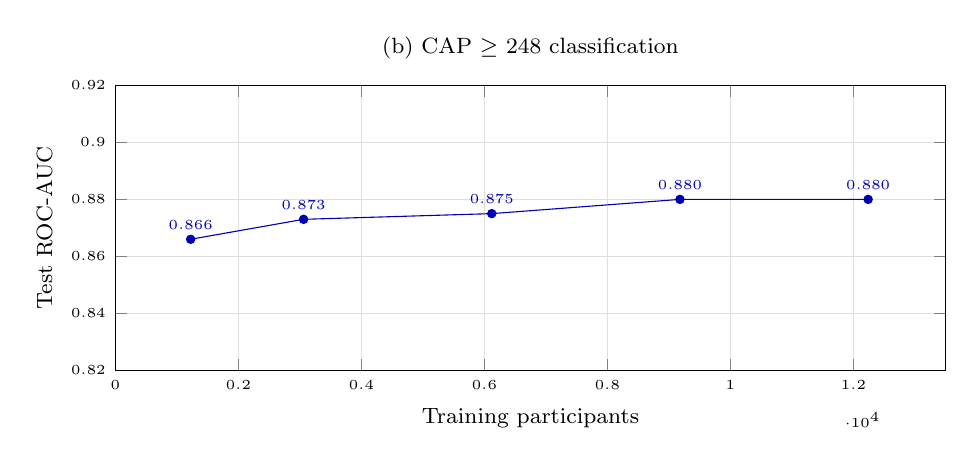
\begin{tikzpicture}
\begin{axis}[
  width=\linewidth, height=5.2cm,
  title={\footnotesize (b) CAP $\geq$ 248 classification},
  xlabel={\footnotesize Training participants}, ylabel={\footnotesize Test ROC-AUC},
  xmin=0, xmax=13500, ymin=0.82, ymax=0.92,
  tick label style={font=\tiny}, label style={font=\footnotesize},
  grid=major, grid style={gray!25},
  nodes near coords={\pgfmathprintnumber[fixed,zerofill,precision=3]{\pgfplotspointmeta}},
  every node near coord/.append style={font=\tiny, above},
  ]
\addplot[blue!70!black, mark=*, mark size=1.5pt]
  coordinates {(1224,0.866) (3060,0.873) (6120,0.875) (9180,0.880) (12240,0.880)};
\end{axis}
\end{tikzpicture}
\end{minipage}
\caption{Learning curve of the selected settings: held-out test $R^2$ and AUC within the scope ($n = 1{,}236$) against the number of training participants. $R^2$ rises from 0.501 with 1,224 participants to 0.556 with 9,180 and only to 0.561 with all 12,240.}
\label{fig:learning-curve}
\end{figure}

Two causes dominate. First, about half of liver fat is genetic: in a prospective twin study the heritability of steatosis measured by MRI-PDFF was 0.52 (95\% CI 0.31--0.73) \cite{loomba2015heritability}. Variants such as \emph{PNPLA3} I148M change liver fat substantially at the same body size, and NHANES 2017--2023 contains no genotypes; lifelong diet, an accurate alcohol history and muscle mass are measured poorly or not at all. Two people with the same weight, waist and blood tests can therefore have very different livers. Second, the model is scored against a single CAP reading. With a reproducibility of about 0.82, a model that even knew about each patient's true liver state could not cross an $R^2$ of the order of 0.8. For routine data, the heritable share and the other unmeasured factors lower the attainable value further, to around 0.6. The in-scope result of 0.562 (0.593 in cross-validation) is close to that ceiling: the plateau is a property of the data, not of the model.

This is also why HepatoTwin relies on the calibrated probabilities of steatosis rather than on the exact CAP value. They discriminate well (AUC 0.88) and are well calibrated, and they outperform the established clinical scores on the same participants.

%--------------------------------------------------------------------
\section{Comparison with Published Models}
\label{sec:exp-compare}

Published models fall into two groups: those predicting a continuous liver-fat value, which report $R^2$, and NHANES models classifying steatosis, which report AUC. No NHANES study reporting $R^2$ for CAP was found, so this work provides the first such benchmark.

\begin{table}[t]
\centering
\small
\caption{Continuous liver-fat prediction from routine data.}
\label{tab:cmp-r2}
\begin{tabularx}{\textwidth}{@{}>{\raggedright\arraybackslash}p{2.9cm} >{\raggedright\arraybackslash}p{2.3cm} >{\raggedright\arraybackslash}p{1.7cm} Y >{\raggedright\arraybackslash}p{2.0cm}@{}}
\toprule
Study & Population & Reference & Inputs & $R^2$ \\
\midrule
UK Biobank \cite{insitro2024ukb} & 40,533 UK adults & MRI-PDFF & 37 body and blood measures & 0.37 \\
UK Biobank \cite{insitro2024ukb} & 9,723 UK adults & MRI-PDFF & Plasma metabolomics & 0.34 \\
UK Biobank \cite{insitro2024ukb} & 46,000 UK adults & MRI-PDFF & DXA images (not routine) & 0.63--0.64 \\
Asaturyan et al.\ \cite{asaturyan2022fli} & 28,796 UK adults & MRI-PDFF & Fatty Liver Index alone & 0.28--0.36 \\
Asaturyan et al.\ \cite{asaturyan2022fli} & As above & MRI-PDFF & 12 variables incl.\ diagnoses & 0.54 \\
Pet\"aj\"a et al.\ \cite{petaja2016igfbp} & 378 Finnish adults & $^{1}$H-MRS & Includes a specialist marker & 0.44 / 0.49$^{c}$ \\
Liu H.\ et al.\ \cite{liu2022surrogate} & 272, obesity clinic & CAP & BMI, neck, TG, C-peptide & 0.63--0.65$^{d}$ \\
Haas et al.\ \cite{haas2021liverfat} & UK Biobank & MRI & BMI and 24 clinical factors & $\approx$0.34$^{e}$ \\
Fatty Liver Index, this cohort & 13,502 / 5,548 & CAP & FLI (linear fit) & 0.44 / 0.50 \\
\textbf{This study} & 15,300 NHANES & CAP & 81 routine inputs & 0.56 test; 0.59 CV \\
\bottomrule
\end{tabularx}
\par\smallskip
\begin{minipage}{\textwidth}
\footnotesize
$^{c}$Adjusted, discovery / validation.
$^{d}$Validation sample of a small, selected cohort with high CAP (median 320--335\,dB/m against 251 in NHANES), which widens the outcome range and raises $R^2$.
$^{e}$Reported as $r = 0.58$.
Kotronen et al.\ \cite{kotronen2009prediction} and Chen et al.\ \cite{chen2023shsi} report no $R^2$.
This study: within the scope; 0.50 for all participants.
\end{minipage}
\end{table}

\begin{table}[t]
\centering
\small
\caption{NHANES steatosis classification models.}
\label{tab:cmp-auc}
\begin{tabularx}{\textwidth}{@{}>{\raggedright\arraybackslash}p{3.0cm} Y Y Y@{}}
\toprule
Study & Outcome & Reported & This study \\
\midrule
Du et al.\ \cite{du2026masld} & MASLD, CAP $\geq$ 280 & AUC 0.815--0.842 & 0.879 (0.868) \\
Liu L.\ et al.\ \cite{liu2024automl} & CAP $\geq$ 302 & AUC 0.859; FLI 0.838 & 0.888 (0.872) \\
Zhang et al.\ \cite{zhang2025masld} & CAP $\geq$ 302 & AUC 0.874 & 0.888 (0.872) \\
Boullion et al.\ \cite{boullion2025biomarker} & CAP $\geq$ 238 & Accuracy 79.6\% & 0.881 (0.857), CAP $\geq$ 248 \\
Zhu et al.\ \cite{zhu2026nonobese} & Asian, BMI $<$ 28 & Macro AUC 0.874 (three grades) & 0.799 test; 0.823 CV \\
\bottomrule
\end{tabularx}
\par\smallskip
{\footnotesize This study: AUC within the scope, with all 3,060 test participants in brackets. The published studies cover adults of all ages, so the bracketed values are the closer comparison.}
\end{table}

Within its scope, the model's held-out $R^2$ of 0.56 (0.59 in cross-validation) is comparable to or above published routine-data models of liver fat (0.34--0.54; Table~\ref{tab:cmp-r2}), including 0.37 in UK Biobank and 0.49 in validation for a spectroscopy equation that needs a specialist blood marker. Across all ages its $R^2$ of 0.50 still exceeds the UK Biobank routine-data model. Higher values come only from a small selected sample (0.65) or from imaging inputs (0.63--0.64). The studies differ in reference measure and population, so these values are indicative rather than directly comparable; the claim that can be made is ``comparable to or above published routine-data models'', not ``state of the art''. In classification the model matches or exceeds every NHANES model (Table~\ref{tab:cmp-auc}). The exception is lean Asian participants, where its AUC (0.80) is below the three-grade macro AUC of Zhu et al.\ (0.874), a metric that is not directly comparable and that rests on a training set of about 150,000 Chinese adults.

%--------------------------------------------------------------------
\section{Summary}
\label{sec:exp-summary}

Fifty-one experiments raised $R^2$ from 0.491 for the first 14-input model to 0.562 on the held-out test set within the model's scope (ages 12 to 59, reliable reference examination), 0.593 in repeated cross-validation, and 0.578 on participants examined two to six years after the training data. Changes of algorithm, features, loss or tuning each moved $R^2$ by about 0.01 or less; the gains came from adding information (more NHANES variables and a second cycle) and from defining the population in which the model is used. The plateau near 0.56--0.59 is set by the data: about half of liver fat is heritable and unmeasured, and CAP is itself a noisy measure. At this level the model is comparable to or above published routine-data models, and its calibrated steatosis probabilities, which HepatoTwin uses, outperform the Fatty Liver Index and the Hepatic Steatosis Index.

The main limitations are that all validation is internal to NHANES; that the final settings were chosen with the help of the test set, which makes the test $R^2$ slightly optimistic; that patients aged 60 and over are outside the scope; and that the data are cross-sectional, so the model describes the current state and cannot by itself predict the response to a change in diet.